\documentclass[10pt]{article}

  \usepackage{pgfplots}
\pgfplotsset{compat=newest}
%% the following commands are needed for some matlab2tikz features
\usetikzlibrary{plotmarks}
\usetikzlibrary{arrows.meta}
\usepgfplotslibrary{patchplots}
\usepackage{grffile}
\usepackage{amsmath}
\usepackage{lineno}


%\usepackage{fullpage}
\usepackage[top=0.0in, bottom=1in, left=0.8in, right=1in]{geometry}
\usepackage{multicol}
\usepackage{caption}
\usepackage{subcaption}
\usepackage{hyperref}
\usepackage{xcolor}
\usepackage{graphicx,psfrag}
\usepackage[pdf]{pstricks}

\definecolor{lightblue}{rgb}{.80,.9,1}
\newcommand{\hl}[1]
    {\par\colorbox{lightblue}{\parbox{\linewidth}{#1}}}

\newcommand{\defn}{\stackrel{\textrm{\scriptsize def}}{=}}

\setlength{\columnsep}{0.01pc}

\title{Non-linear dispersive water wave models}
\author{Jordan Pitt}
\date{}

% TIME ON EVERY PAGE AS WELL AS THE FILE NAME
\usepackage{fancyhdr}
\usepackage{currfile}
\usepackage[us,12hr]{datetime} % `us' makes \today behave as usual in TeX/LaTeX
\pagestyle{plain}

\definecolor{mycolor1}{rgb}{0.00000,0.44700,0.74100}%
\definecolor{mycolor2}{rgb}{0.85000,0.32500,0.09800}%
\definecolor{mycolor3}{rgb}{0.92900,0.69400,0.12500}%
\definecolor{mycolor4}{rgb}{0.49400,0.18400,0.55600}%
\definecolor{mycolor5}{rgb}{0.46600,0.67400,0.18800}% 
\definecolor{mycolor6}{rgb}{0.30100,0.74500,0.93300}%
\definecolor{mycolor7}{rgb}{0.63500,0.07800,0.18400}%

\newcommand\T{\rule{0pt}{3ex }}       % Top table strut
\newcommand\B{\rule[-4ex]{0pt}{4ex }} % Bottom table strut

\newcommand\TM{\rule{0pt}{2.8ex }}       % Top matrix strut
\newcommand\BM{\rule[-2ex]{0pt}{2ex }} % Bottom matrix strut

\newcommand{\vecn}[1]{\boldsymbol{#1}}
\DeclareRobustCommand{\solidrule}[1][0.25cm]{\rule[0.5ex]{#1}{1.5pt}}

\DeclareRobustCommand{\dashedrule}{\mbox{%
		\solidrule[2mm]\hspace{2mm}\solidrule[2mm]}}

\DeclareRobustCommand{\tikzcircle}[1]{\tikz{\filldraw[#1] (0,0) circle (0.5ex);}}	
	
	
\DeclareRobustCommand{\squaret}[1]{\tikz{\draw[#1,thick] (0,0) rectangle (0.2cm,0.2cm);}}
\DeclareRobustCommand{\circlet}[1]{\tikz{\draw[#1,thick] (0,0) circle [radius=0.1cm];}}
\DeclareRobustCommand{\trianglet}[1]{\tikz{\draw[#1,thick] (0,0) --
		(0.25cm,0) -- (0.125cm,0.25cm) -- (0,0);}}
\DeclareRobustCommand{\crosst}[1]{\tikz{\draw[#1,thick] (0cm,0cm) --
		(0.1cm,0.1cm) -- (0cm,0.2cm) -- (0.1cm,0.1cm) -- (0.2cm,0.2cm) -- (0.1cm,0.1cm)-- (0.2cm,0cm);}}
\DeclareRobustCommand{\diamondt}[1]{\tikz{\draw[#1,thick] (0,0) --(0.1cm,0.15cm) -- (0.2cm,0cm) -- (0.1cm,-0.15cm) -- (0,0)  ;}}
\DeclareRobustCommand{\squareF}[1]{\tikz{\filldraw[#1,fill opacity= 0.3] (0,0) rectangle (0.2cm,0.2cm);}}

\begin{document}
\maketitle
\begin{figure}[h!]
	\centering
	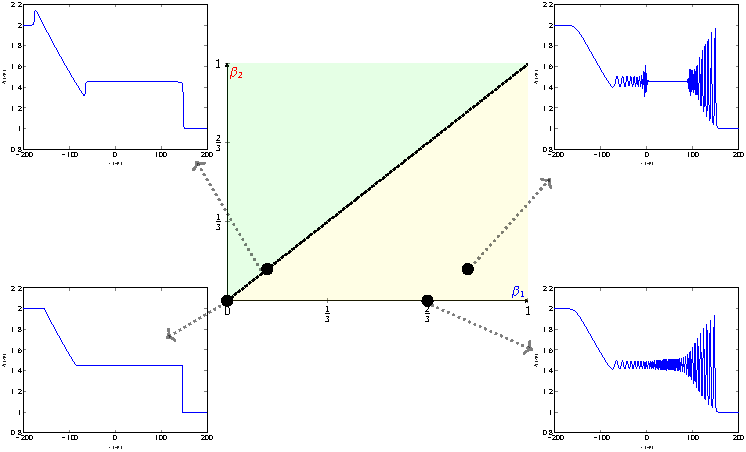
\includegraphics[width=1\textwidth]{3x3Grid.pdf}
	\caption{Example numerical solutions for water depth ($h$) to the dam break problem for the generalised Serre-Green-Naghdi equations}
\end{figure}
In this talk we discuss the family of equations described by the generalised Serre-Green-Naghdi equations which model water waves using the water depth ($h$), the depth-averaged horizontal velocity ($u$) and the acceleration due to gravity ($g$). There are two free parameters ${\color{blue} {\beta_1}}$ and ${\color{red} {\beta_2}}$ which allow the dispersion properties of the equations to be changed. The generalised Serre-Green-Naghdi equations for one spatial dimension ($x$) are given by
\begin{align*}
&\dfrac{\partial h}{\partial t} + \dfrac{\partial (hu)}{\partial x} = 0\\
&\dfrac{\partial (hu)}{\partial t} + \dfrac{\partial }{\partial x} \left( hu^2 + \frac{1}{2}gh^2  +  {\color{blue} {\beta_1} \Phi } -   {\color{red} {\beta_2}\Psi}  \right)= 0 \\
\end{align*}
where
\begin{align*}
\color{blue} \Phi  & \color{blue}= \frac{h^3}{2}\left( \frac{\partial u}{\partial x}\frac{\partial u}{\partial x} - \frac{\partial^2 u}{\partial x \partial t} - u\frac{\partial^2 u}{\partial x^2}\right) \\
\color{red} \Psi & \color{red}=  \frac{gh^2}{2} \left(h \frac{\partial^2 h}{\partial x^2} + \frac{1}{2} \frac{\partial h}{\partial x}\frac{\partial h}{\partial x}\right)
\end{align*}
The focus of the talk will be introducing these equations and comparing the numerical solutions to the dam-break problem (stationary Riemann problem) displayed in Figure 1 to the linear theory. 


\end{document} 